\documentclass[tikz,border=4pt]{standalone}
\usepackage[T1]{fontenc}
\usepackage{lmodern}
\renewcommand{\familydefault}{\sfdefault}
\usetikzlibrary{shapes.geometric,positioning,arrows.meta,calc,fit,backgrounds,decorations.pathreplacing}
\tikzset{
  node distance=6mm,
  every node/.style={font=\footnotesize,align=center,execute at begin node={\hyphenpenalty=10000\relax}},
  base/.style={draw=gray!60,fill=gray!12,minimum height=7mm,inner sep=2pt},
  term/.style={base,rounded corners=3.5mm,text width=30mm},
  proc/.style={base,text width=32mm},
  err/.style={base,text width=30mm,fill=gray!22},
  io/.style={base,trapezium,trapezium left angle=72,trapezium right angle=108,trapezium stretches=true,text width=28mm},
  dec/.style={base,diamond,aspect=2.4,text width=27mm,inner sep=0pt},
  % predefined process: a call to another procedure
  sub/.style={proc,inner xsep=3mm,path picture={
    \draw[gray!60] ([xshift=1.5mm]path picture bounding box.north west)--([xshift=1.5mm]path picture bounding box.south west)
                   ([xshift=-1.5mm]path picture bounding box.north east)--([xshift=-1.5mm]path picture bounding box.south east);}},
  go/.style={-{Stealth[length=2mm]},draw=gray!55!black},
  lab/.style={font=\scriptsize,fill=white,inner sep=1pt},
  frame/.style={draw=gray!60,dashed,rounded corners=2mm,inner sep=3mm},
  % memory diagrams
  cell/.style={draw=gray!60,fill=gray!12,minimum height=7mm,inner sep=1pt,font=\scriptsize},
  hot/.style={cell,fill=gray!35},
  note/.style={font=\scriptsize,text=gray!30!black},
}

\begin{document}
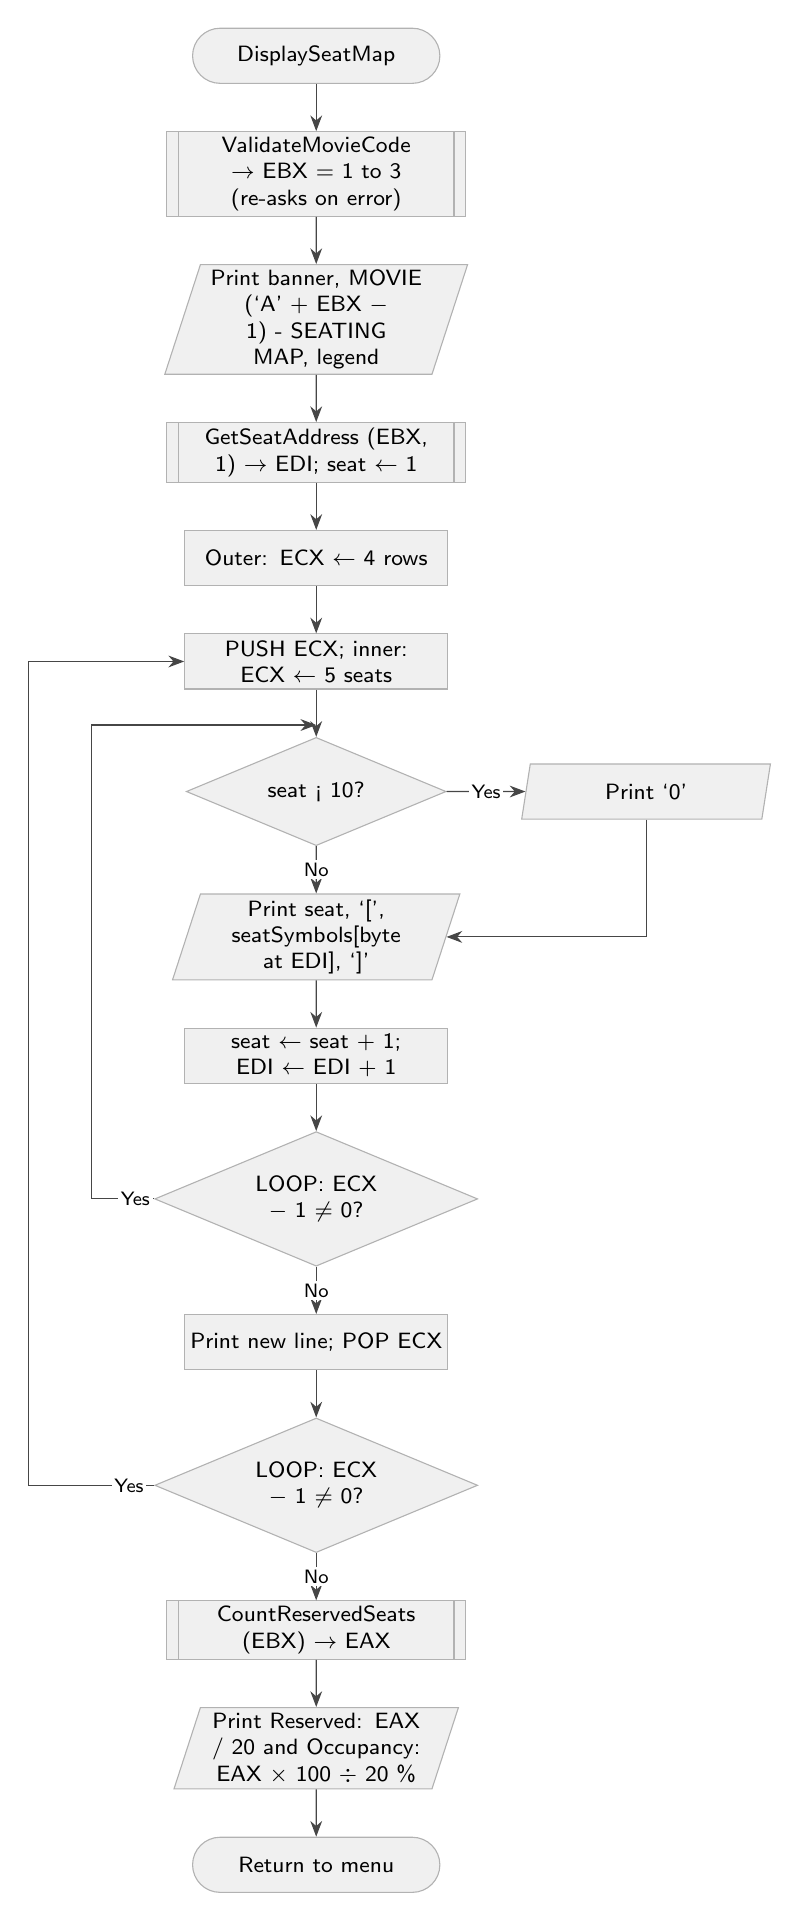
\begin{tikzpicture}
\node[term] (s) {DisplaySeatMap};
\node[sub,below=of s] (v) {ValidateMovieCode $\rightarrow$ EBX = 1 to 3 (re-asks on error)};
\node[io,below=of v] (t) {Print banner, MOVIE (`A' + EBX $-$ 1) - SEATING MAP, legend};
\node[sub,below=of t] (g) {GetSeatAddress (EBX, 1) $\rightarrow$ EDI; seat $\leftarrow$ 1};
\node[proc,below=of g] (o) {Outer: ECX $\leftarrow$ 4 rows};
\node[proc,below=of o] (i) {PUSH ECX; inner: ECX $\leftarrow$ 5 seats};
\node[dec,below=of i] (d1) {seat < 10?};
\node[io,right=10mm of d1] (z) {Print `0'};
\node[io,below=of d1] (p) {Print seat, `[', seatSymbols[byte at EDI], `]'};
\node[proc,below=of p] (n) {seat $\leftarrow$ seat + 1; EDI $\leftarrow$ EDI + 1};
\node[dec,below=of n] (l1) {LOOP: ECX $-$ 1 $\neq$ 0?};
\node[proc,below=of l1] (nl) {Print new line; POP ECX};
\node[dec,below=of nl] (l2) {LOOP: ECX $-$ 1 $\neq$ 0?};
\node[sub,below=of l2] (c) {CountReservedSeats (EBX) $\rightarrow$ EAX};
\node[io,below=of c] (r) {Print Reserved: EAX / 20 and Occupancy: EAX $\times$ 100 $\div$ 20 \%};
\node[term,below=of r] (e) {Return to menu};
\draw[go] (s)--(v);
\draw[go] (v)--(t);
\draw[go] (t)--(g);
\draw[go] (g)--(o);
\draw[go] (o)--(i);
\draw[go] (i)--(d1);
\draw[go] (d1)--node[lab]{Yes}(z);
\draw[go] (z)|-(p.east);
\draw[go] (d1)--node[lab]{No}(p);
\draw[go] (p)--(n);
\draw[go] (n)--(l1);
\draw[go] (l1.west)--node[lab,pos=.3]{Yes}++(-8mm,0)|-([yshift=1.5mm]d1.north);
\draw[go] (l1)--node[lab]{No}(nl);
\draw[go] (nl)--(l2);
\draw[go] (l2.west)--node[lab,pos=.2]{Yes}++(-16mm,0)|-(i.west);
\draw[go] (l2)--node[lab]{No}(c);
\draw[go] (c)--(r);
\draw[go] (r)--(e);
\end{tikzpicture}
\end{document}
